%!TEX program = xelatex
\documentclass[11pt,a4paper]{article}
\usepackage[utf8]{inputenc}
\usepackage[T1]{fontenc}
\usepackage{authblk}
\usepackage{tikz}
\usepackage{pgfplots}
\usepackage{verbatim}
\usepackage{amsfonts}
\usepackage{amsmath}
\usepackage{amsthm}
\usepackage{indentfirst}
\usepackage{amssymb}
\setlength{\parindent}{0pt}
\usetikzlibrary{shapes,snakes}
\newcommand{\argmax}{\operatornamewithlimits{argmax}}
\newcommand{\argmin}{\operatornamewithlimits{argmin}}
\DeclareMathOperator{\col}{col}
\usepackage{booktabs}
\newtheorem{theorem}{Theorem}
\newtheorem{note}{Note}
\newtheorem{definition}{Definition}
\newtheorem{proposition}{Proposition}
\newtheorem{lemma}{Lemma}
\newtheorem{example}{Example}
\newtheorem{corollary}{Corollary}
\usepackage{graphicx}
\usepackage{geometry}
\usepackage{hyperref}
\newcommand{\code}{	exttt}
\geometry{a4paper,scale=0.8}
\title{STAT 425 Final Project}
\author[*]{Wenxiao Yang}
\affil[*]{Department of Mathematics, University of Illinois at Urbana-Champaign}
\date{2021}
\begin{document}
\maketitle

\section{Introduction}
This project aims to identify the optimal operating conditions for Company XX's bubble wrap lines in order to increase production capacity. We investigate the results of a completely randomized design experiment. There are two factors: \textit{line speed} (with three levels, $36,37,38 m/mm$), \textit{percent loading of additives} (with three levels, $0,2,4\%$). And one response: \textit{production rate} ($lbs/hr$). The experiment was replicated three times.\\
Our goal is to find the \textbf{optimal combination} of \textit{line speed} and \textit{percent load of additives} that results in the \textbf{highest production rate}.


\section{Analysis}
The goal of our regression analysis is to fit a two-way ANOVA model to determine the effects of various factors with different levels. We started with the full model, which included the effects of various factors as well as the interaction term.

\subsection{Full Model: Significance}
The full factor effects model is as follows:
$$Y_{ijk}=\mu+\alpha_i+\beta_j+(\alpha\beta)_{ij}+\varepsilon_{ijk}$$
$Y_{ijk}$: \textit{Production rate} for \textit{Line Speed} $i$, \textit{Percent Loading of Additives} $j$, \textit{replication} $k$.\\
$\alpha_i$: effect of \textit{Line Speed} $i$ on \textit{Production rate}.\\
$\beta_j$: effect of \textit{Percent Loading of Additives} $j$ on \textit{Production rate}.\\
$(\alpha\beta)_{ij}$: interaction term.\\
The error terms satisfy the usual assumption $\varepsilon_{i j k} \sim \mathcal{N}\left(0, \sigma^{2}\right)$.\\
Sum Constraints: $\sum_{i} \alpha_{i}=0, \sum_{j} \beta_{j}=0, \sum_{i}(\alpha \beta)_{i j}=\sum_{j}(\alpha \beta)_{i j}=0$.\\
$i=36,37,38.$\\
$j=0\%,2\%,4\%.$\\
$k=1,2,3$\\

We first plot the Interaction Plots (Figure 1) and then use the partial F-test of ANOVA table (Figure 2) to test the interaction term's significance.\\
We find the interaction is presented in the plot. However, the p-value (0.68293) of the F-test is higher than 0.05, we conclude that the interaction terms are not statistically significant. So, we can remove it from the model.\\
\begin{figure}[htb]
    \centering
    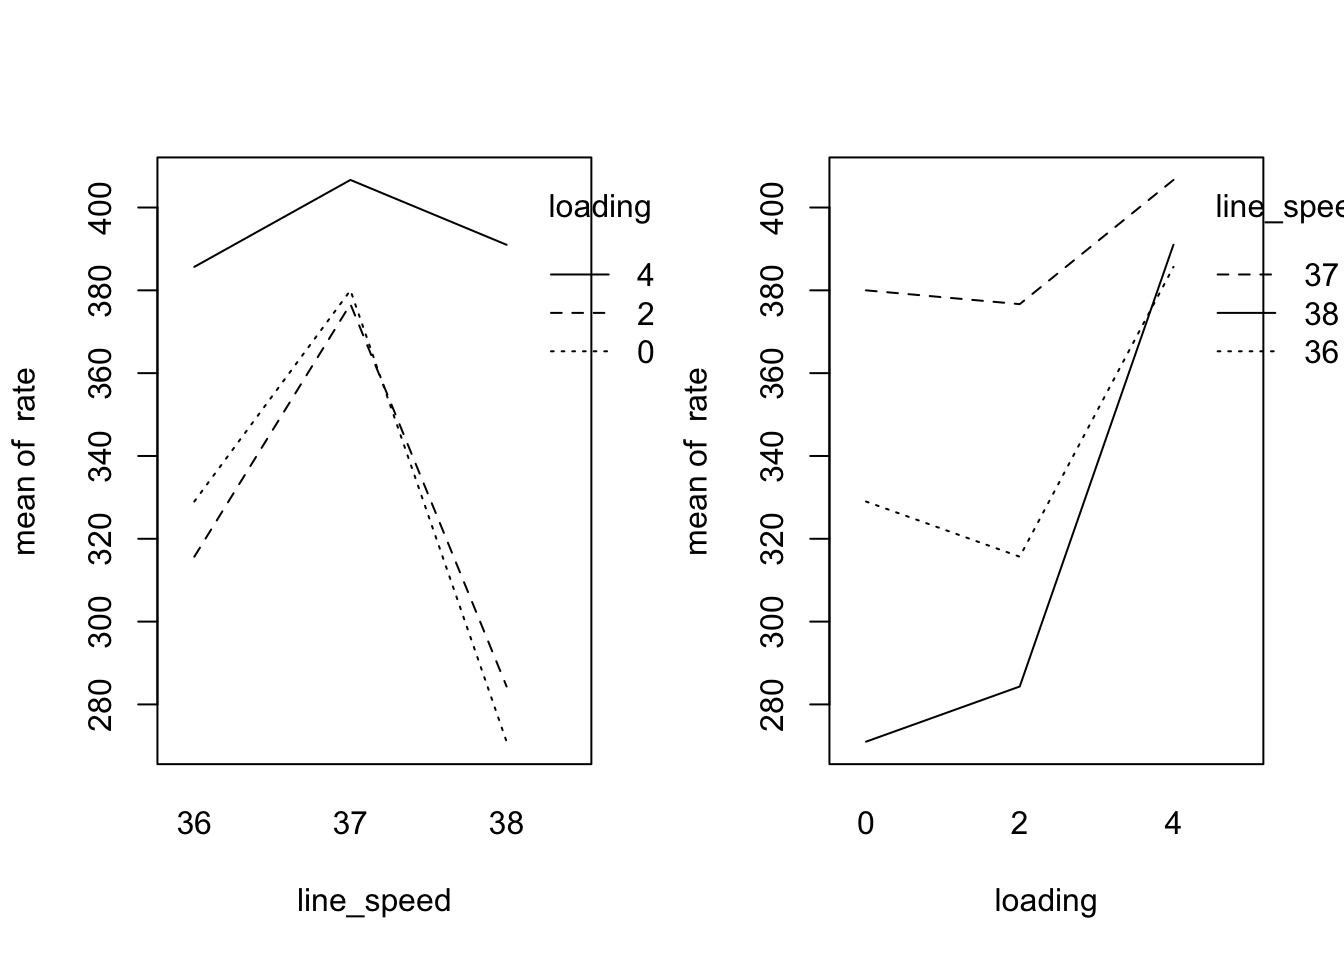
\includegraphics[scale=0.3]{inter1.png}
    \caption{Interaction Plots}
    \label{}
\end{figure}
\begin{figure}[htb]
    \centering
    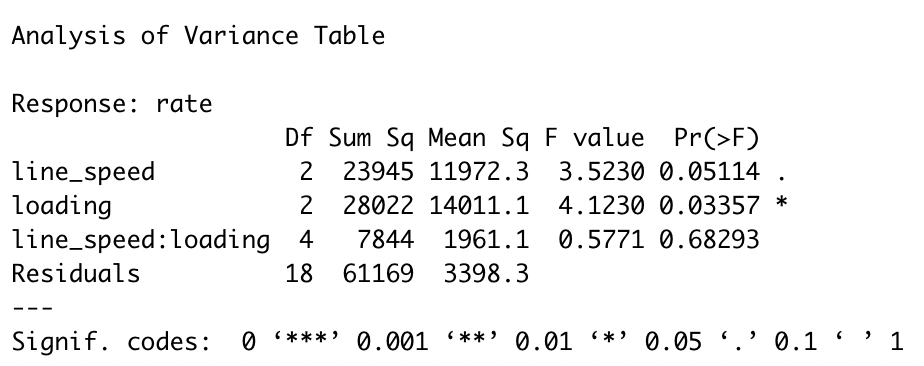
\includegraphics[scale=0.8]{inter2.png}
    \caption{ANOVA Table: Full model}
    \label{}
\end{figure}


\subsection{Additive Model: Significance}
Then we fit the regression of the additive model:
$$Y_{ijk}=\mu+\alpha_i+\beta_j+\varepsilon_{ijk}$$
$Y_{ijk}$: \textit{Production rate} for \textit{Line Speed} $i$, \textit{Percent Loading of Additives} $j$, \textit{replication} $k$.\\
$\alpha_i$: effect of \textit{Line Speed} $i$ on \textit{Production rate}.\\
$\beta_j$: effect of \textit{Percent Loading of Additives} $j$ on \textit{Production rate}.\\
The error terms satisfy the usual assumption $\varepsilon_{i j k} \sim \mathcal{N}\left(0, \sigma^{2}\right)$.\\
Sum Constraints: $\sum_{i} \alpha_{i}=0, \sum_{j} \beta_{j}=0$.\\
$i=36,37,38.$\\
$j=0\%,2\%,4\%.$\\
$k=1,2,3$\\

We use the partial F-test of the ANOVA table (Figure 3) to test the significance of both factors. Since the p-values of both factors are lower than 0.05 (\textit{Line Speed}: 0.03777, \textit{Percent Loading of Additives}: 0.02355), we can conclude that both factors are statistically significant.
\begin{figure}[htb]
    \centering
    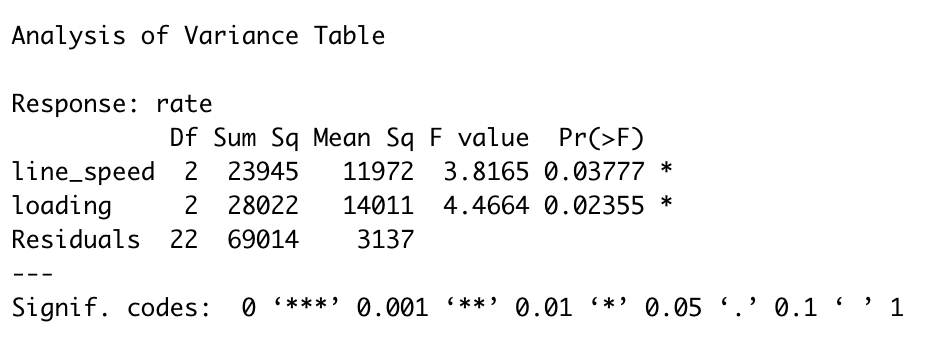
\includegraphics[scale=0.8]{add1.png}
    \caption{ANOVA Table: Additive Model}
    \label{}
\end{figure}

\subsection{Additive Model: Check Assumptions}
Then we need to check the assumptions of the additive model.\\
We plot the diagnostic plots (Figure 4) which includes 1. Residuals vs. Fitted plot; 2. Normal Q-Q plot.\\
1. Constancy of Variance (Homoscedasticity): In the Residuals vs. Fitted plot, the points scatter equally. \\

\begin{center}\begin{figure}[htb]
    \centering
    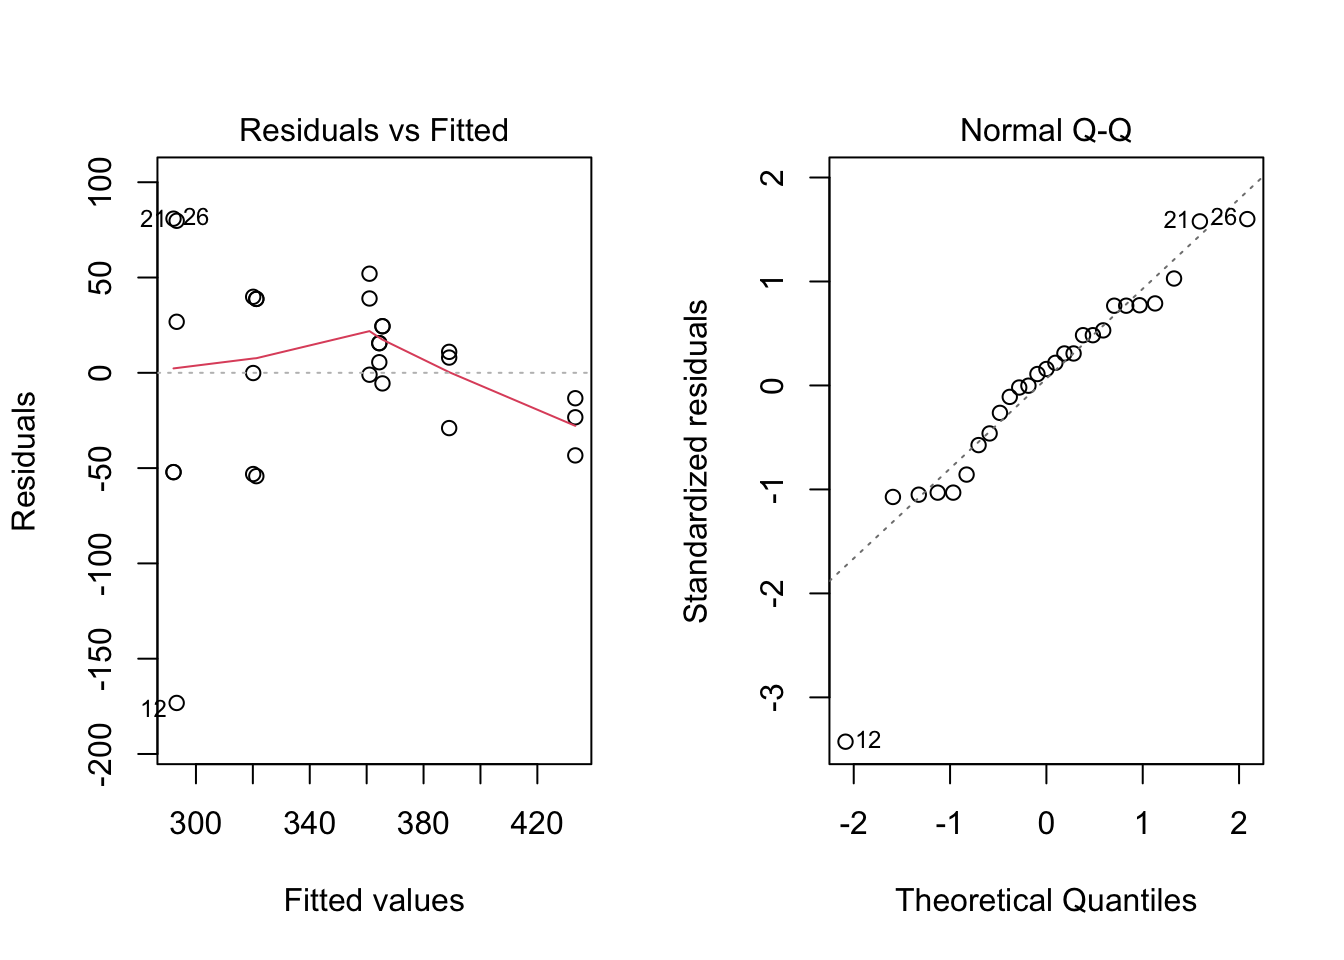
\includegraphics[scale=0.3]{DP1}
    \caption{}
    \label{}
\end{figure}\end{center}











\end{document}